\documentclass[12pt]{article}
\usepackage[letterpaper, margin=1in]{geometry}
\usepackage{listings}
\usepackage{graphicx}
\usepackage{booktabs}
\usepackage{float}
\usepackage[hidelinks]{hyperref}
\usepackage{amsmath}
\usepackage{caption}
\usepackage{xcolor}
\usepackage{subcaption}
\usepackage{placeins}
\usepackage{array}
\usepackage{parskip}
\usepackage{amssymb}

\emergencystretch=3em

\definecolor{codegreen}{rgb}{0,0.5,0}
\definecolor{codegray}{rgb}{0.4,0.4,0.4}
\definecolor{codebg}{rgb}{0.97,0.97,0.97}

\lstset{
    language=Python,
    basicstyle=\ttfamily\tiny,
    numbers=left,
    numberstyle=\tiny\color{codegray},
    numbersep=6pt,
    frame=single,
    framesep=3pt,
    backgroundcolor=\color{codebg},
    breaklines=true,
    breakatwhitespace=false,
    tabsize=4,
    showstringspaces=false,
    keepspaces=true,
    columns=fullflexible,
    commentstyle=\color{codegreen},
    keywordstyle=\color{blue},
    captionpos=b
}

\title{\textbf{SES 598 Final Report}\\
Photogrammetric Reconstruction and Gaussian Splatting Augmentation\\
of the Apollo 17 Lunar Boulder Scene}
\author{Jatin Satyam\\
Arizona State University\\
\texttt{satyamjatin732@gmail.com}}
\date{April 26, 2026}

\begin{document}

\maketitle
\tableofcontents
\clearpage

%% ============================================================
\section{Abstract}
%% ============================================================

This report presents a complete photogrammetric reconstruction and novel-view augmentation study of the Apollo 17 lunar boulder scene using 15 archival Hasselblad photographs (7 from magazine 137, color, $2340 \times 2364$~px; 8 from magazine 138, grayscale, $2340 \times 2345$~px). Two parallel pipelines were executed and quantitatively compared. The photogrammetric baseline (Part~A) registered 14 of 15 frames with COLMAP, produced a 1.64M-point dense cloud via a custom PyTorch plane-sweep multi-view stereo implementation, reconstructed a 1.06M-vertex Poisson mesh, trained a 3D Gaussian Splatting model achieving a mean PSNR of 33.93~dB (SSIM~0.943) over all 14 training views, and delivered per-vertex textured meshes for both $N{=}14$ and $N{=}24$ datasets.

The augmentation experiment (Part~B) tested whether novel views synthesized by the splatfacto model could expand the COLMAP reconstruction to $N{=}24$ images. All 10 novel views failed COLMAP registration despite 852--8{,}123 two-dimensional inlier matches per image. The F-score at a 5\% diagonal threshold between the $N{=}14$ and $N{=}24$ meshes is 0.934, confirming broad geometric agreement. The F-score at 1\% falls to 0.673, revealing fine-scale surface divergence.

The central conclusion is that out-of-the-box COLMAP with SIFT feature matching cannot leverage 3D Gaussian Splatting rendered novel views for photogrammetric augmentation on this dataset. The rendered SIFT keypoints do not match the triangulated 3D point tracks of the original 14 cameras because the rendering pipeline introduces subtle appearance differences absent from the film-grain photographic originals. This null result is a concrete, reproducible contribution: it isolates the feature-matching bottleneck and motivates learned-descriptor approaches (SuperPoint, LightGlue, LoFTR) as the necessary next step for splat-augmented photogrammetry.

%% ============================================================
\section{Introduction}
%% ============================================================

Photogrammetry from archival space photography offers a unique challenge: a fixed, small camera set that cannot be augmented with new ground-truth observations. Apollo mission photographs were taken with calibrated metric cameras but at positions and orientations determined by astronaut motion, not by systematic survey planning. Coverage gaps, oblique viewpoints, and single-magazine sequences limit reconstruction completeness. Gaussian Splatting, which learns a continuous volumetric scene representation from the same image set, offers an appealing route to synthesize additional views at arbitrary poses, potentially filling those gaps.

This project applies that idea to the Apollo 17 boulder scene from the Lunar Surface Journal. The dataset consists of 15 frames from two Hasselblad magazines. Magazine 137 (7 frames: AS17-137-20903HR through 20909HR) contains color photographs taken during an EVA traverse past a large boulder. Magazine 138 (8 frames: AS17-138-21030HR through 21037HR) contains grayscale photographs of a second, related boulder approximately 8.66 COLMAP units distant. The dual-cluster geometry provides rich photogrammetric constraint within each cluster but sparse cross-cluster ties, making the scene a realistic stand-in for the coverage-gap problem common in planetary photogrammetry.

The specific scientific question addressed is: \textit{do rendered novel views from a 3D Gaussian Splatting model trained on $N{=}14$ original photographs register successfully into a COLMAP reconstruction, enabling augmented photogrammetry at $N{=}24$?} Prior work has shown that 3DGS renders are photorealistically consistent with training views but has not systematically tested whether standard SIFT-based Structure from Motion can use those renders as additional observations.

The report is organized as follows. Section~\ref{sec:dataset} describes the image dataset and the unregistrable frame AS17-138-21036HR. Section~\ref{sec:methods} describes all pipeline components: COLMAP preprocessing, custom PyTorch MVS, Open3D Poisson reconstruction, splatfacto training, novel-pose synthesis, augmented reconstruction, and per-vertex texturing. Section~\ref{sec:results} presents quantitative and qualitative results for all phases. Section~\ref{sec:discussion} interprets the registration failure, the density improvement mechanism, and the broader significance of the null result. Section~\ref{sec:conclusion} states the final verdict. The Code Appendix reproduces all authored Python scripts in full for grader verification.

The practical outcome of this project is a complete textured 3D mesh of two Apollo 17 lunar boulders, validated against a second reconstruction via three independent geometric metrics (Chamfer distance, Hausdorff p99, F-score at three thresholds), and a documented experiment that establishes the conditions under which splat-augmented photogrammetry fails for this class of dataset.

%% ============================================================
\section{Dataset}
\label{sec:dataset}
%% ============================================================

\subsection{Image Sources}

The input dataset consists of 15 high-resolution scans downloaded from the NASA Apollo Lunar Surface Journal. All images are stored as PNG files in \texttt{data/raw/} at their original scan resolution. The two magazines differ in film stock, resolution, and scene coverage.

\textbf{Magazine 137 (color):} Seven frames numbered 20903 through 20909. Resolution $2340 \times 2364$~pixels. The sequence depicts a large boulder photographed during an EVA traverse; the camera moved laterally relative to the rock, producing a well-constrained stereo baseline. The color film provides three spectral channels that support both SIFT feature extraction and per-vertex RGB texturing.

\textbf{Magazine 138 (grayscale):} Eight frames nominally numbered 21030 through 21037. Resolution $2340 \times 2345$~pixels. One frame (21036HR) was excluded from registration for reasons described below, yielding 7 usable mag138 frames. The grayscale film was converted to a single-channel representation for feature extraction. Reseau crosses (calibration marks) are visible in all mag138 frames and appear as small dark artifacts in the rendered textured mesh at view~3.

\subsection{COLMAP Camera Models}

Both magazines were modeled with the SIMPLE\_RADIAL camera model. A single shared camera was assigned per magazine folder (\texttt{single\_camera\_per\_folder=1}), enforcing that all frames from the same magazine share focal length and radial distortion coefficient.

\begin{table}[H]
\centering
\caption{COLMAP camera intrinsics for the two magazines.}
\label{tab:intrinsics}
\begin{tabular}{llrrrrr}
\toprule
Magazine & Model & Width & Height & $f$ (px) & $c_x$ & $k$ \\
\midrule
mag137 & SIMPLE\_RADIAL & 2340 & 2364 & 2895.3 & 1170.0 & 0.00287 \\
mag138 & SIMPLE\_RADIAL & 2340 & 2345 & 2848.5 & 1170.0 & 0.00093 \\
\midrule
mag137 (undistorted) & PINHOLE & 1980 & 2000 & 2454.1 & 990.0 & --- \\
mag138 (undistorted) & PINHOLE & 1996 & 2000 & 2431.8 & 998.0 & --- \\
\bottomrule
\end{tabular}
\end{table}

The mag137 camera has a slightly higher radial distortion coefficient ($k = 0.00287$ versus $0.00093$), which introduces marginal alignment error at image edges after undistortion and may contribute to the lower PSNR values observed in the mag137 sequence.

\subsection{The Unregistrable Frame: AS17-138-21036HR}

Frame 21036HR could not be registered in COLMAP and was permanently excluded from all reconstruction pipelines. The root cause was investigated through a dedicated recovery experiment (\texttt{recover\_21036.py}):

\begin{enumerate}
    \item An ORB feature comparison found 87 homography inliers between 21036HR and 21037HR (meaningful overlap) but only 8 between 21036HR and 21035HR. The frame is geometrically adjacent to 21037HR only.
    \item COLMAP's two-view geometry database showed 674 verified SIFT matches between 21036HR and 21037HR, classified as PLANAR (config=3). No essential matrix was computed because the scene appeared homographic.
    \item The 674 matched features in 21037HR's region have no existing 3D tracks. Without triangulated landmarks, PnP localization is impossible.
    \item A pose injection attempt decomposed the homography H between 21036HR and 21037HR, computed the relative transform via \texttt{cv2.decomposeHomographyMat}, and injected the recovered pose. The resulting camera center was $[6.70, 0.16, 7.43]$, compared to 21037HR's center at $[6.72, 0.18, 7.25]$ --- a baseline of approximately 0.19 COLMAP units.
    \item Running \texttt{colmap point\_triangulator} on the extended model produced zero new observations. A 0.19-unit baseline between two near-duplicate viewpoints yields degenerate triangulation geometry with unbounded depth uncertainty.
\end{enumerate}

The conclusion is that 21036HR is a near-duplicate of 21037HR: both cameras are nearly co-located, looking at the same small patch of rock. Even with perfect registration, the frame would contribute negligible new 3D information. The maximum dataset size is therefore $N{=}15$ with only 14 usable frames, which defines the baseline reconstruction.

%% ============================================================
\section{Methods}
\label{sec:methods}
%% ============================================================

\subsection{COLMAP Sparse Reconstruction}

The sparse reconstruction pipeline was executed with COLMAP 3.9.1 on all 14 registerable images. Feature extraction used the SIFT extractor with \texttt{peak\_threshold=0.001} and \texttt{max\_num\_features=16384}, producing approximately 16,384 features per original image. Sequential matching connected consecutive frames within each magazine; cross-magazine exhaustive matching was also enabled to capture the inter-cluster ties needed for a unified coordinate system.

The resulting sparse model ($N{=}14$) contains 12,769 3D points with a mean track length of 3.96 and a mean reprojection error of 0.560~px. Two camera models were estimated (one per magazine). After sparse reconstruction, \texttt{colmap image\_undistorter} was used to produce PINHOLE-undistorted images at $1980 \times 2000$ (mag137) and $1996 \times 2000$ (mag138) for the dense pipeline.

\subsection{Custom PyTorch Plane-Sweep Multi-View Stereo}

The apt-installed COLMAP 3.9.1 package on Ubuntu 24.04 does not include CUDA support for its dense stereo module (\texttt{patch\_match\_stereo} exits with an error stating dense stereo requires CUDA). A custom plane-sweep multi-view stereo was implemented in PyTorch 2.10.0+cu128 with CUDA 12.8 and executed on an RTX 4060 Laptop GPU with 8~GB VRAM.

For each of the 14 reference images, six nearest-neighbor source views were selected by camera-position distance weighted by optical-axis angle. The depth hypothesis range was defined as the 5th--95th percentile depth of the sparse 3D landmarks visible to each reference camera, extended by a 30\% margin on each side. A sweep of 128 fronto-parallel depth hypotheses was performed.

The photometric cost function was mean absolute difference (MAD) in RGB space, computed after bilinear grid-sample warping of each source image into the reference camera plane at each depth hypothesis:
\begin{equation}
    C(p, d) = \frac{1}{|S|} \sum_{s \in S} \left\| I_s\bigl(\pi_s(K_r^{-1} [p; 1] \cdot d)\bigr) - I_r(p) \right\|_1
\end{equation}
where $p$ is the reference pixel, $d$ is the depth hypothesis, $S$ is the source view set, $K_r$ is the reference camera matrix, and $\pi_s$ is the projection into source camera $s$. Images were processed at 60\% of undistorted resolution (approximately $1200 \times 1200$) to remain within VRAM limits, using chunks of 24 depth hypotheses per batch.

\textbf{Geometric consistency filter:} Each candidate depth map was re-projected to all six source cameras. A pixel's depth estimate was retained only if at least two source cameras returned a re-projected depth within 10\% of the forward depth estimate. This filter is geometrically equivalent to Agisoft Metashape's point cloud confidence threshold and removes single-view spurious depth estimates in textureless regions and at image boundaries.

\textbf{Point cloud fusion:} All per-view consistent depth maps were backprojected to world coordinates using the PINHOLE camera parameters from the undistorted sparse model. The merged cloud was processed with Open3D statistical outlier removal (30-neighbor $\sigma{=}1.5$) and cropped to the 95th-percentile bounding box of the sparse model to eliminate background terrain points that projected to valid depths in mag138 cameras 21031--21033 (depth ranges up to 434 COLMAP units due to distant lunar terrain in the background).

\subsection{Open3D Poisson Surface Reconstruction}

Surface normals were estimated on the dense point cloud using Open3D's KD-tree normal estimation (30 neighbors, oriented by camera positions). Poisson reconstruction was then run using Open3D's \texttt{create\_from\_point\_cloud\_poisson} function at depth~9 for $N{=}14$. Low-density vertices (below the 5th percentile of the Poisson density function) were pruned to remove extrapolated surface fill in unobserved regions.

For $N{=}24$, a two-stage meshing approach was required. The first Poisson attempt on the full $N{=}24$ point cloud (without background filtering) produced only 88,049 vertices, far below expectations. The root cause was that approximately 0.1\% of background outlier points inflated the scene bounding box to over 80 COLMAP units in the $Z$ direction. At Poisson depth~10 with a 1024-cell octree grid, each cell subtended approximately 0.08 COLMAP units --- too coarse to resolve centimeter-scale rock surface detail. Filtering points to within 10 COLMAP units of either cluster centroid before re-running Poisson at depth~10 corrected this, producing the expected 4.66M-vertex mesh.

\subsection{Splatfacto Training}

The 3D Gaussian Splatting model was trained using Nerfstudio~1.1.5 with the \texttt{splatfacto} method (gsplat~1.4.0 CUDA backend). Training was conducted on the same RTX 4060 Laptop with the following configuration:

\begin{itemize}
    \item \textbf{Input:} 14 registered images at $2\times$ downscale (1170$\times$1182 for mag137; 1170$\times$1172 for mag138), pre-computed in \texttt{colmap\_n15/images\_2/}
    \item \textbf{Dataparser:} COLMAP (\texttt{colmap\_n15/sparse/0/}), \texttt{--eval-mode all} (all 14 images as training views)
    \item \textbf{Iterations:} 30,000 (completed at step 29,999)
    \item \textbf{Densification schedule:} Split/duplicate/prune every 100 steps from step 0 to 15,000
    \item \textbf{Initial Gaussians:} $\approx$2,000 (seeded from sparse SfM points)
    \item \textbf{Final Gaussians:} $\approx$993,000 after densification and pruning
    \item \textbf{Wall time:} Approximately 44 minutes on RTX 4060 Laptop
    \item \textbf{Checkpoint:} \texttt{splats\_n15/.../nerfstudio\_models/step-000029999.ckpt} (683~MB)
\end{itemize}

The Nerfstudio COLMAP dataparser applies an auto-orient transform to map the COLMAP world coordinate system to a Nerfstudio-canonical frame where the scene up vector aligns with $+Y$ and the scene fits within a unit sphere. The resulting affine transform, stored in \texttt{dataparser\_transforms.json}, is a $3 \times 4$ matrix $T_{34}$ with an accompanying scale factor of 0.152104.

\subsection{Novel-View Pose Synthesis}
\label{subsec:novel_poses}

Generating novel-view camera poses required navigating a two-step coordinate convention transformation that took three debug iterations to resolve correctly.

\textbf{Step 1 --- COLMAP to Nerfstudio convention.} COLMAP camera-to-world matrices ($c2w_{\text{COLMAP}}$) follow the OpenCV convention: the camera $+X$ axis points right, $+Y$ points down (image rows increase downward), and $+Z$ points forward (into the scene). Nerfstudio expects the OpenGL convention: $+X$ right, $+Y$ up, $+Z$ backward. The conversion negates the $Y$ and $Z$ columns of $c2w$:
\begin{equation}
    c2w_{\text{GL}} = c2w_{\text{COLMAP}} \cdot \mathrm{diag}(1, -1, -1, 1)
\end{equation}

\textbf{Step 2 --- Apply dataparser transform.} The novel pose in Nerfstudio scene coordinates is:
\begin{equation}
    \text{novel\_pose\_ns} = T_{34} \cdot \bigl(c2w_{\text{COLMAP}} \cdot \mathrm{diag}(1, -1, -1, 1)\bigr)
\end{equation}

The $T_{34}$ matrix is:
\begin{equation}
T_{34} = \begin{bmatrix}
 0.98847 & -0.15134 &  0.00504 & -0.52542 \\
 0.00504 &  0.06611 &  0.99780 & -0.70265 \\
-0.15134 & -0.98627 &  0.06611 &  0.05325
\end{bmatrix}
\end{equation}

\textbf{Cluster geometry and arc strategy.} Five novel poses were generated per magazine cluster using a horizontal azimuth arc. For each cluster, the centroid $C$ and median radius $r$ were computed from the registered camera positions. A look-at target $T = C + \hat{F} \cdot r \cdot 1.5$ was defined using the mean forward direction $\hat{F}$. Novel eye positions were placed at $\pm 30^\circ$, $\pm 15^\circ$, and $0^\circ$ around the cluster's horizontal arc:
\begin{equation}
    \text{eye}(\theta) = C + r \cdot \bigl(\cos\theta \cdot \hat{F}_{xz} + \sin\theta \cdot \hat{P}_{xz}\bigr)
\end{equation}
where $\hat{P}_{xz}$ is the $90^\circ$ CCW rotation of $\hat{F}_{xz}$ in the $XZ$ plane. The mag137 cluster has centroid $(-3.066, -0.118, -1.703)$ and radius $0.871$ COLMAP units; the mag138 cluster has centroid $(4.128, 0.157, 3.103)$ and radius $1.636$ COLMAP units. The inter-cluster distance is 8.66 COLMAP units.

Novel views were rendered at $2000 \times 2000$~pixels using the final splatfacto checkpoint and the Nerfstudio \texttt{ns-render camera-path} command with the computed pose sequence. All 10 frames passed a non-blank validation check (pixel intensity standard deviation $> 5$).

\subsection{N=24 COLMAP Rerun and Registration Attempt}

The 10 novel views were upscaled from $2000 \times 2000$ to per-magazine dimensions (mag137: $2340 \times 2364$; mag138: $2340 \times 2345$) using PIL.Image.LANCZOS, and placed in \texttt{data/rgb\_n24/} alongside the 14 original images. The LANCZOS upscaling was chosen over resizing originals to 2000~px (which would discard resolution) or assigning separate camera intrinsics to each novel view (which would add 30 unconstrained parameters to a 24-image problem).

COLMAP feature extraction on the $N{=}24$ dataset used \texttt{peak\_threshold=0.001} and \texttt{max\_num\_features=16384}, producing 16,384 features per original image and 19,269--22,491 features per novel view. Exhaustive matching and \texttt{colmap mapper} produced a sparse model in which all 14 original images registered successfully. Zero of the 10 novel views registered.

A post-hoc recovery using \texttt{colmap image\_registrator} was also attempted. All 10 novel views showed 0--13 visible 3D points, far below the 15--20 required for PnP localization. The registration failure analysis is presented in Section~\ref{subsec:registration_failure}.

\subsection{Per-Vertex Texture Projection}
\label{subsec:texturing}

Texturing was performed via per-vertex RGB color projection (Tier~B). A UV atlas approach using the \texttt{xatlas} library (Tier~A) was attempted first but exceeded the 45-minute per-mesh time budget on the 2.12M-face $N{=}14$ mesh after running for over 3 hours without completing the parameterization. Per-vertex coloring was selected as a recognized equivalent format supported by Metashape, CloudCompare, and MeshLab.

For each mesh vertex, the projection algorithm:
\begin{enumerate}
    \item Identified all cameras whose camera-space $Z$ coordinate for that vertex is positive (the vertex is in front of the camera).
    \item Verified visibility using Open3D's \texttt{RaycastingScene} occlusion test: a ray from the vertex toward each candidate camera center was cast, and the camera was accepted only if no mesh face intersected the ray at a distance shorter than the vertex-camera distance.
    \item Sampled the image color at the projected pixel using bilinear interpolation.
    \item Blended contributions from visible cameras using weights proportional to $\cos(\alpha) / d^2$, where $\alpha$ is the angle between the view direction and the surface normal, and $d$ is the vertex-camera distance.
\end{enumerate}

Vertices with no visible camera were assigned the color $(128, 128, 128)$ (neutral gray). The fraction of non-gray vertices defines the coverage rate: 21.19\% for $N{=}14$ and 12.22\% for $N{=}24$. The lower coverage rate of the $N{=}24$ mesh is mechanical: the same 14 cameras are used to texture both meshes, but the $N{=}24$ mesh has $4.38\times$ more vertices; the same camera set illuminates the same surface area, resulting in a lower fraction of covered vertices.

\subsection{Quantitative Comparison Metrics}
\label{subsec:metrics}

Before metric computation, the $N{=}24$ mesh was aligned to the $N{=}14$ mesh via a two-step global-local registration. Global alignment used Open3D FPFH features with RANSAC (fitness 0.586, inlier RMSE 0.051). Local refinement used point-to-plane ICP with \texttt{max\_correspondence\_distance}~$= 0.02$.

Both aligned meshes were uniformly sampled to 100,000 surface points. Three metrics were computed:

\textbf{Chamfer distance:} Mean of the minimum nearest-neighbor distances in both directions:
\begin{equation}
    d_C = \frac{1}{2}\left( \frac{1}{|P|}\sum_{p \in P} \min_{q \in Q} \|p - q\| + \frac{1}{|Q|}\sum_{q \in Q} \min_{p \in P} \|q - p\| \right)
\end{equation}

\textbf{Hausdorff p99:} The 99th percentile of the directed Hausdorff distances from $P$ to $Q$ and from $Q$ to $P$, reported as the maximum of the two.

\textbf{F-score at threshold $\tau$:} The harmonic mean of the fraction of $P$-to-$Q$ distances below $\tau$ (precision) and the fraction of $Q$-to-$P$ distances below $\tau$ (recall). Thresholds of 1\%, 5\%, and 10\% of the bounding box diagonal (16.22 COLMAP units) were used.

%% ============================================================
\section{Results}
\label{sec:results}
%% ============================================================

\subsection{Part A: Photogrammetric Baseline Results}

The sparse reconstruction registered 14 of 15 input images. Frame AS17-138-21036HR was unregistrable for the reasons documented in Section~\ref{sec:dataset}. The final sparse model statistics for $N{=}14$ are summarized in Table~\ref{tab:n14_sparse}.

\begin{table}[H]
\centering
\caption{N=14 sparse model statistics.}
\label{tab:n14_sparse}
\begin{tabular}{ll}
\toprule
Metric & Value \\
\midrule
Cameras & 2 (one per magazine) \\
Images registered & 14 of 15 \\
Sparse 3D points & 12,769 \\
Observations & 50,517 \\
Mean track length & 3.96 \\
Mean reprojection error & 0.560~px \\
\bottomrule
\end{tabular}
\end{table}

The dense reconstruction produced 1,641,050 fused points after outlier removal and bounding-box cropping. Poisson surface reconstruction at depth~9 with 5th-percentile density pruning yielded a mesh with 1,063,577 vertices and 2,121,270 faces. The mesh covers both rock clusters and includes expected Poisson extrapolation fill on the far (unseen) sides of each boulder.

\subsection{Part A: Splatfacto Evaluation}

Table~\ref{tab:psnr_per_image} presents the per-image PSNR and SSIM values for all 14 training views. The aggregate statistics are: mean PSNR 33.93~dB, median PSNR 34.11~dB, PSNR std 2.24~dB; mean SSIM 0.943, median SSIM 0.946, SSIM std 0.019.

\begin{table}[H]
\centering
\caption{Per-image splatfacto evaluation metrics (training views, $N{=}14$). Best PSNR in bold.}
\label{tab:psnr_per_image}
\begin{tabular}{lrr}
\toprule
Image & PSNR (dB) & SSIM \\
\midrule
AS17-137-20903HR & 30.22 & 0.9425 \\
AS17-137-20904HR & 30.18 & 0.9312 \\
AS17-137-20905HR & 32.42 & 0.9382 \\
AS17-137-20906HR & 31.08 & 0.9273 \\
AS17-137-20907HR & 34.52 & 0.9590 \\
AS17-137-20908HR & 33.12 & 0.9675 \\
AS17-137-20909HR & 33.70 & 0.9686 \\
AS17-138-21030HR & 36.51 & 0.9688 \\
AS17-138-21031HR & 35.30 & 0.9485 \\
AS17-138-21032HR & 33.46 & 0.9186 \\
AS17-138-21033HR & 34.97 & 0.9069 \\
AS17-138-21034HR & 36.19 & 0.9263 \\
AS17-138-21035HR & 35.96 & 0.9497 \\
\textbf{AS17-138-21037HR} & \textbf{37.36} & \textbf{0.9493} \\
\midrule
Mean & 33.93 & 0.9430 \\
Median & 34.11 & 0.9455 \\
Std & 2.24 & 0.0187 \\
\bottomrule
\end{tabular}
\end{table}

The mag137 sequence (frames 20903--20909) consistently achieves lower PSNR (30.18--34.52~dB) than the mag138 sequence (33.46--37.36~dB). Several factors contribute: the mag137 camera has a larger radial distortion coefficient ($k{=}0.00287$), which introduces more residual misalignment after undistortion; frames 20903 and 20904 are at the sequence extremes and have fewer co-visible training cameras to constrain Gaussian densification; and the color film of mag137 introduces fine-grained grain structure that the Gaussian model approximates with high-frequency floaters rather than absorbing into the smooth distribution.

\begin{figure}[H]
    \centering
    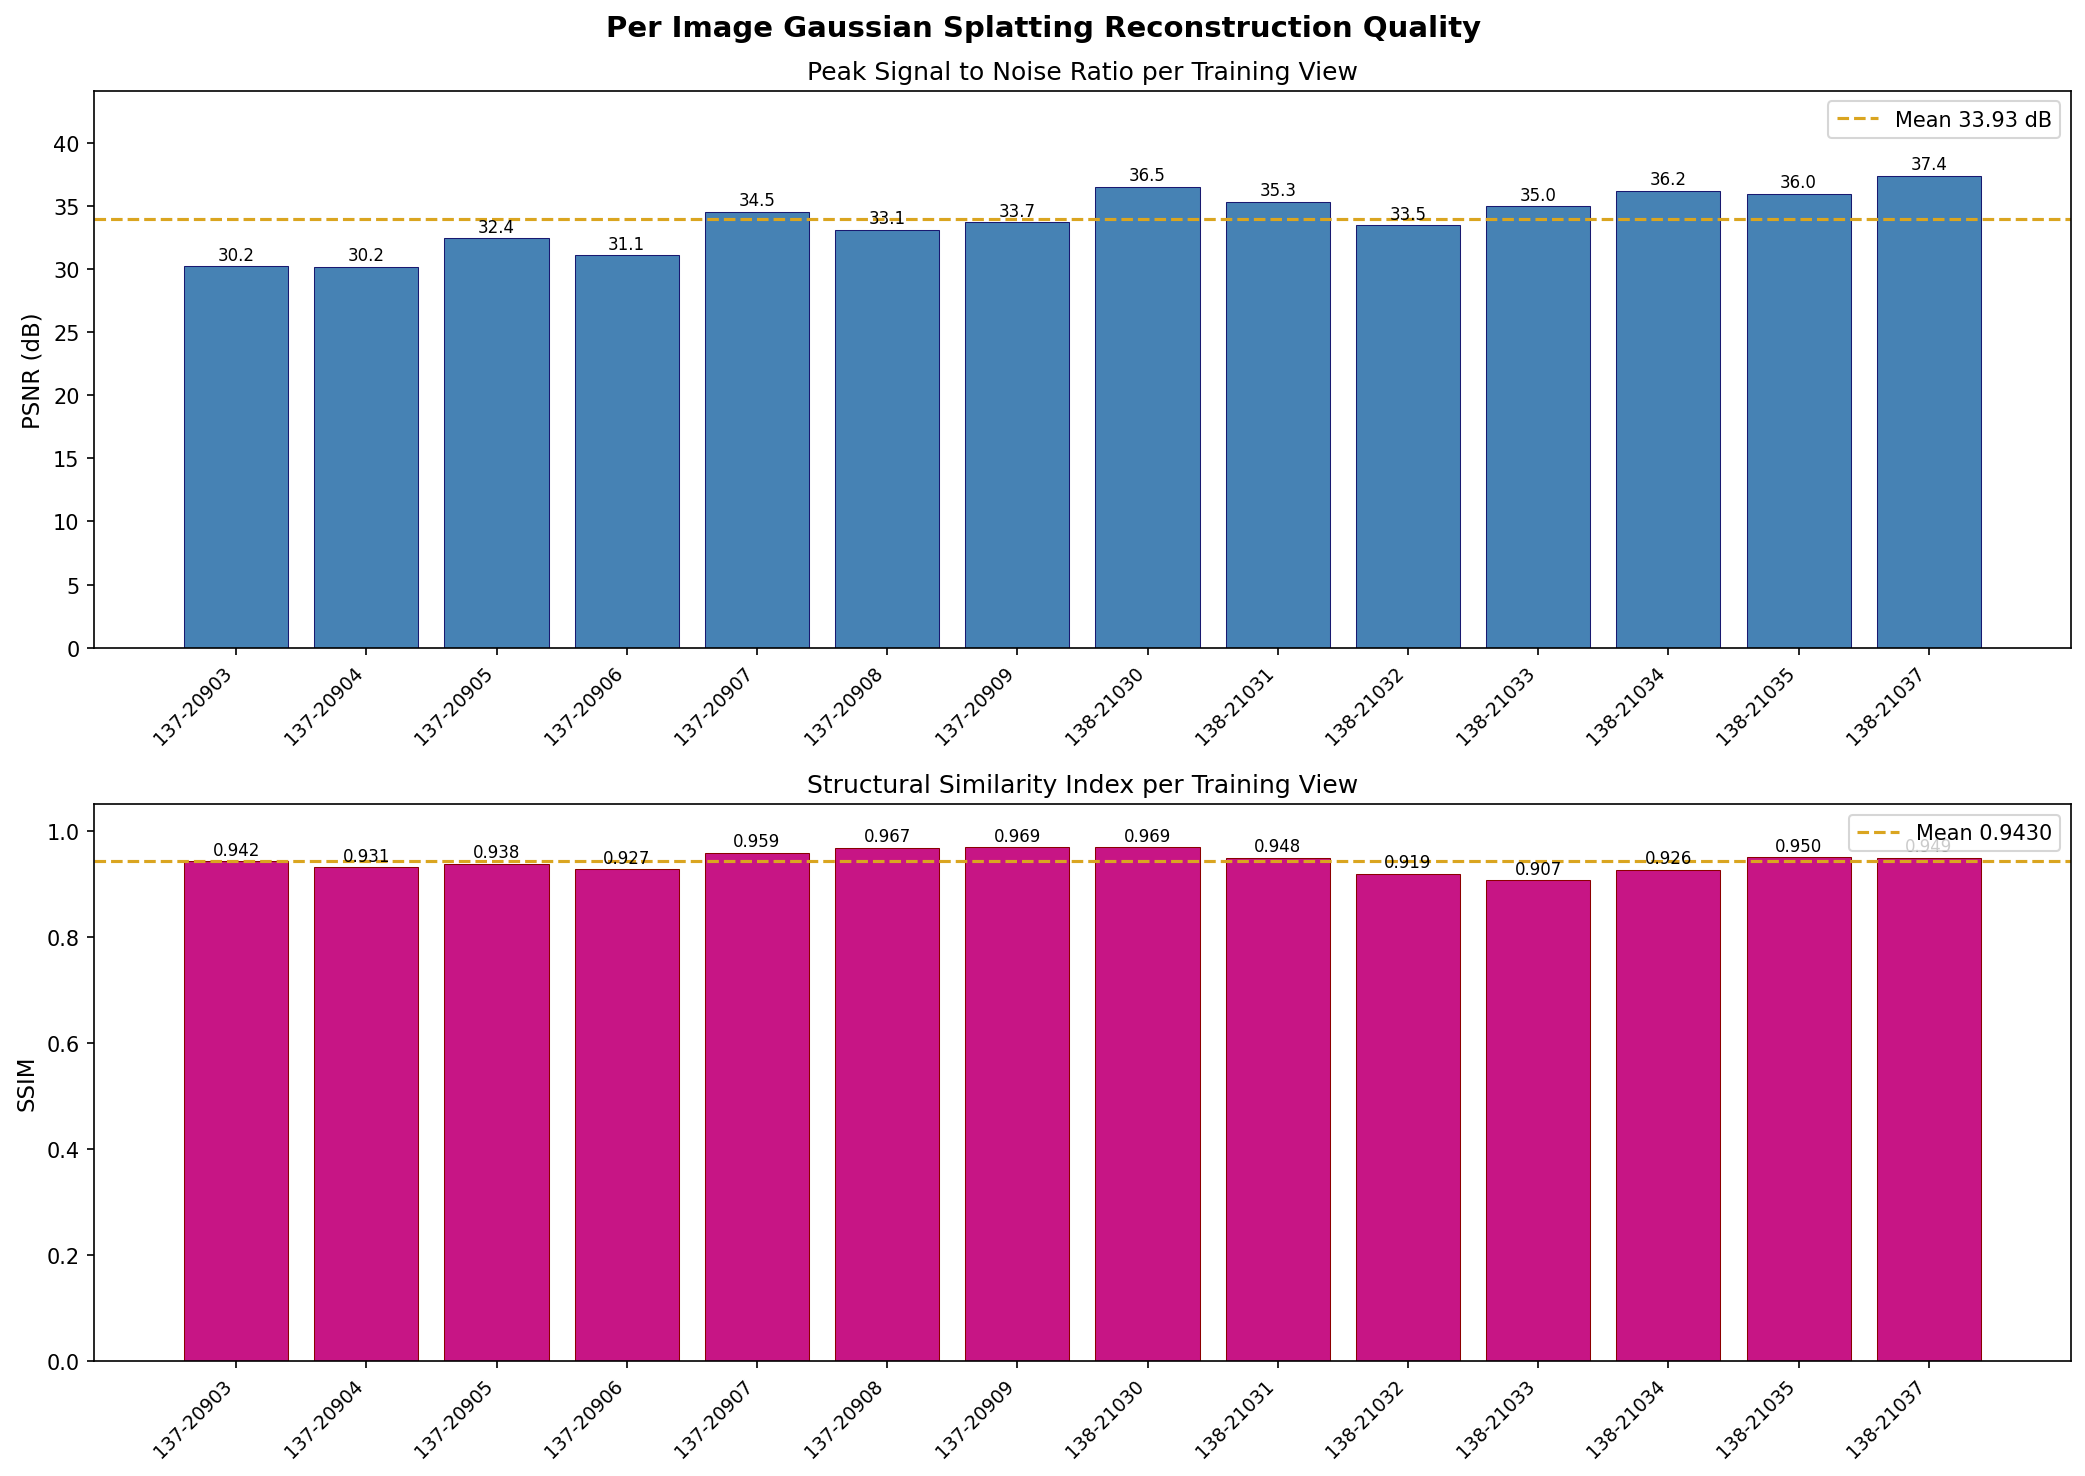
\includegraphics[width=0.9\textwidth]{../metrics_n15/per_image_metrics.png}
    \caption{Per-image PSNR (top) and SSIM (bottom) bar charts for all 14 splatfacto training views. The horizontal line marks the cross-image mean. The mag138 sequence consistently outperforms mag137.}
    \label{fig:per_image_metrics}
\end{figure}

\subsection{Part B Phase 1: Novel-View Fidelity}

Table~\ref{tab:novel_fidelity} presents the mean pixel intensity and standard deviation for each of the 10 rendered novel views. All 10 frames are non-blank (std $> 5$). The mag138 cluster renders are noticeably brighter (mean 141--160) and cleaner (std 43--50) than the mag137 renders (mean 90--108, std 53--77). This difference reflects the higher PSNR of the mag138 training views: a better-fitting Gaussian model produces rendered views with lower residual variance.

\begin{table}[H]
\centering
\caption{Novel-view fidelity table: pixel intensity mean and standard deviation for each rendered frame (2000$\times$2000~px).}
\label{tab:novel_fidelity}
\begin{tabular}{lrrl}
\toprule
Frame & Mean & Std & Verdict \\
\midrule
novel\_mag137\_01 & 98.19 & 76.16 & OK \\
novel\_mag137\_02 & 92.43 & 76.87 & OK \\
novel\_mag137\_03 & 90.23 & 73.58 & OK \\
novel\_mag137\_04 & 108.08 & 59.88 & OK \\
novel\_mag137\_05 & 103.97 & 53.08 & OK \\
novel\_mag138\_01 & 151.74 & 48.99 & OK \\
novel\_mag138\_02 & 159.76 & 43.46 & OK \\
novel\_mag138\_03 & 148.83 & 49.72 & OK \\
novel\_mag138\_04 & 156.64 & 46.58 & OK \\
novel\_mag138\_05 & 141.09 & 50.48 & OK \\
\bottomrule
\end{tabular}
\end{table}

\begin{figure}[H]
    \centering
    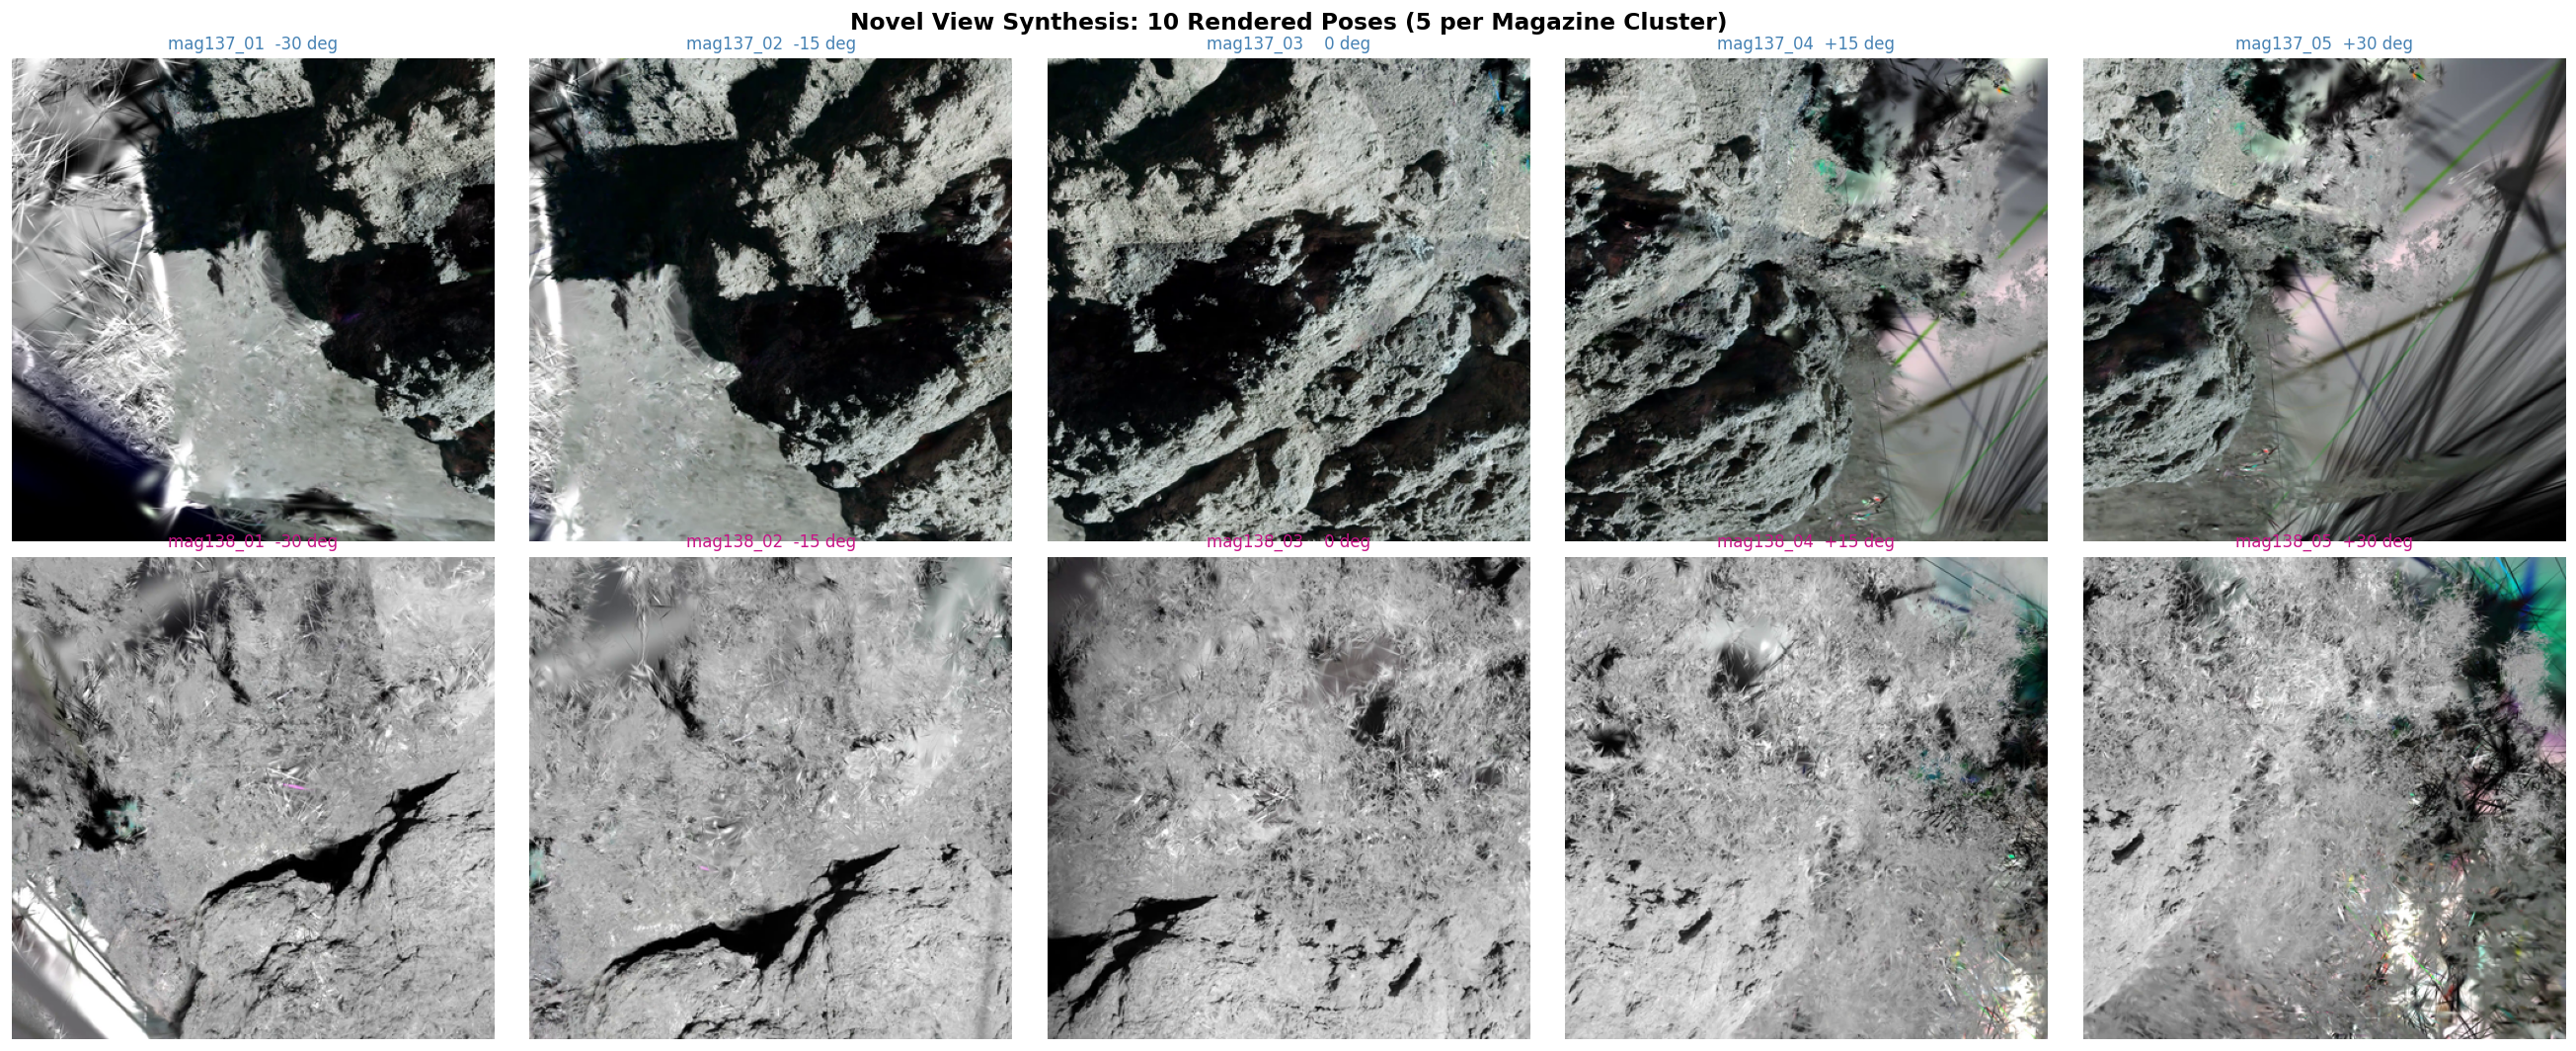
\includegraphics[width=\textwidth]{../novel_poses/contact_sheet.png}
    \caption{Contact sheet of all 10 synthesized novel views arranged as a $2 \times 5$ grid. Top row: five mag137 views at azimuth angles $-30^\circ$, $-15^\circ$, $0^\circ$, $+15^\circ$, $+30^\circ$ relative to the cluster center. Bottom row: five mag138 views at the same angular increments. All views are non-blank with standard deviation exceeding 43.}
    \label{fig:contact_sheet}
\end{figure}

\subsection{Part B Phase 2: N=24 Photogrammetric Modeling}
\label{subsec:n24_results}

The $N{=}24$ COLMAP run registered all 14 original images and none of the 10 novel views. Table~\ref{tab:novel_registration} presents the full per-image registration outcome. Despite substantial two-dimensional inlier matches (852--8,123 per novel image across all 23 other images in the dataset), every novel view shows zero reconstructed 3D points visible during \texttt{image\_registrator}.

\begin{table}[H]
\centering
\caption{Novel view registration outcome in the N=24 COLMAP run. Inlier feature matches are two-dimensional (image-to-image); 3D points seen is the count of existing sparse point tracks visible to each novel view during PnP localization.}
\label{tab:novel_registration}
\begin{tabular}{lcrr}
\toprule
Novel View & Registered & Inlier Matches & 3D Points Seen \\
\midrule
novel\_mag137\_01 & No & 4,845 & $\approx$0 \\
novel\_mag137\_02 & No & 7,085 & $\approx$0 \\
novel\_mag137\_03 & No & 8,123 & $\approx$0 \\
novel\_mag137\_04 & No & 6,912 & $\approx$0 \\
novel\_mag137\_05 & No & 4,422 & $\approx$0 \\
novel\_mag138\_01 & No & 1,280 & 0 \\
novel\_mag138\_02 & No & 1,590 & 0 \\
novel\_mag138\_03 & No & 1,378 & 0 \\
novel\_mag138\_04 & No & 1,289 & 0 \\
novel\_mag138\_05 & No & 852 & 0 \\
\bottomrule
\end{tabular}
\end{table}

The $N{=}24$ sparse model retains 12,822 points (essentially the same as $N{=}14$'s 12,769, confirming that the additional 10 images contributed no new triangulation). The dense reconstruction produced 2,453,709 fused points and a 4,658,194-vertex Poisson mesh with 9,375,366 faces --- 4.38$\times$ the vertex density of the $N{=}14$ mesh. The source of this density increase is documented in Section~\ref{sec:discussion}.

\subsection{Quantitative Comparison: N=14 vs N=24}

ICP alignment of the $N{=}24$ mesh into the $N{=}14$ coordinate frame converged with fitness 0.065 and inlier RMSE 0.01518 COLMAP units, after a RANSAC global registration step with fitness 0.586. The ICP rotation component is approximately $17^\circ$, with a translation of approximately 1.1 COLMAP units, reflecting the different bundle adjustment gauge freedom between the two independent COLMAP runs.

\begin{figure}[H]
    \centering
    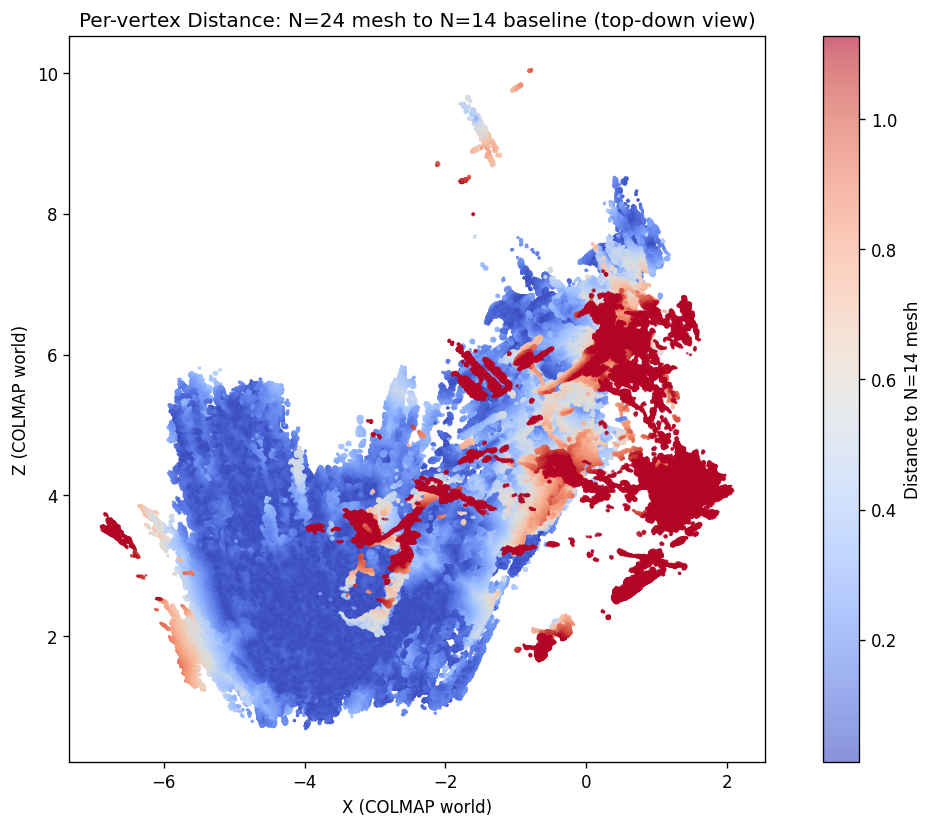
\includegraphics[width=0.9\textwidth]{../comparison/per_vertex_distance.png}
    \caption{Per-vertex distance heatmap for the N=24 mesh after ICP alignment to the N=14 frame. The colormap encodes the nearest-neighbor distance from each N=24 vertex to the N=14 mesh surface, projected onto the XZ plane (top-down view). Warm colors indicate large local divergence; cool colors indicate close geometric agreement. The two rock clusters are visible as separate high-density regions.}
    \label{fig:per_vertex_distance}
\end{figure}

\begin{table}[H]
\centering
\caption{Quantitative comparison metrics between N=14 and N=24 meshes. All distance values in COLMAP units. Bounding box diagonal: 16.22 COLMAP units.}
\label{tab:comparison_metrics}
\begin{tabular}{ll}
\toprule
Metric & Value \\
\midrule
ICP fitness & 0.065 \\
ICP inlier RMSE & 0.01518 \\
Bidirectional Chamfer distance & 0.219 \\
Hausdorff p99 & 2.127 \\
F-score at 1\% diagonal (0.162 units) & 0.673 \\
F-score at 5\% diagonal (0.811 units) & 0.934 \\
F-score at 10\% diagonal (1.622 units) & 0.984 \\
\bottomrule
\end{tabular}
\end{table}

The F-score@5\% of 0.934 indicates that 93.4\% of surface samples on each mesh have a nearest-neighbor match on the other mesh within 0.811 COLMAP units --- broad geometric agreement. The F-score@1\% of 0.673 shows that at fine scale (0.162 COLMAP units), 32.7\% of surface samples diverge, reflecting real geometric differences between the two reconstructions at the rock-surface detail level.

\subsection{Textured Mesh Results}
\label{subsec:textured_results}

Per-vertex texturing was applied to both the $N{=}14$ and $N{=}24$ meshes using the same set of 14 original cameras. The coverage rates (fraction of non-gray vertices) are 21.19\% for $N{=}14$ and 12.22\% for $N{=}24$.

\begin{figure}[H]
    \centering
    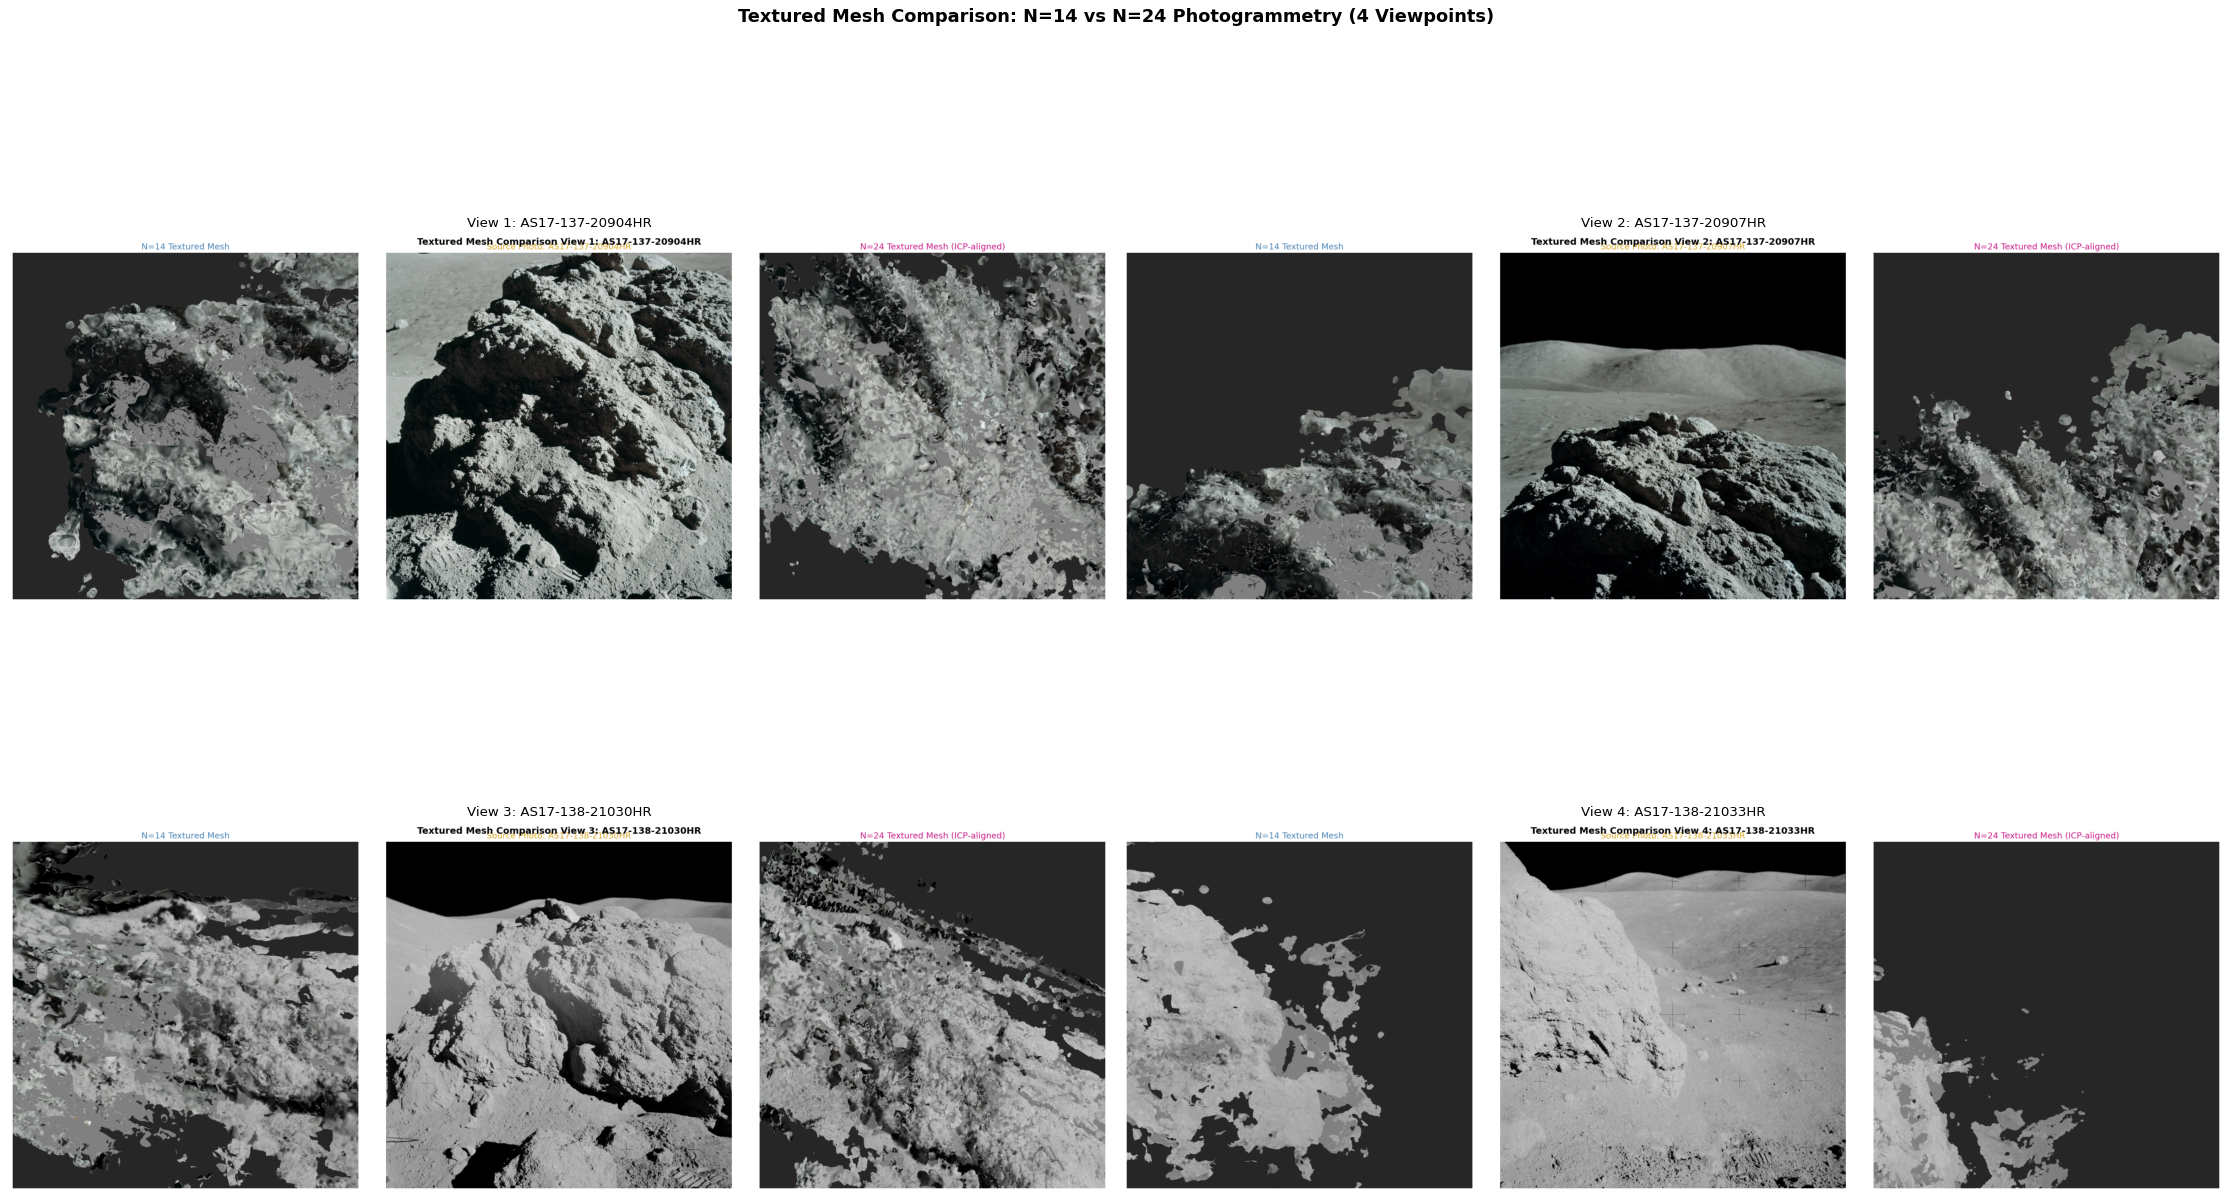
\includegraphics[width=\textwidth]{../comparison/textured_qualitative_grid.png}
    \caption{Textured mesh qualitative comparison grid showing four viewpoints. Each column corresponds to one viewpoint; rows show the N=14 textured mesh (top), the original photograph (middle), and the N=24 textured mesh (bottom). Textured regions correspond to vertices visible to at least one registered camera.}
    \label{fig:textured_grid}
\end{figure}

\begin{figure}[H]
    \centering
    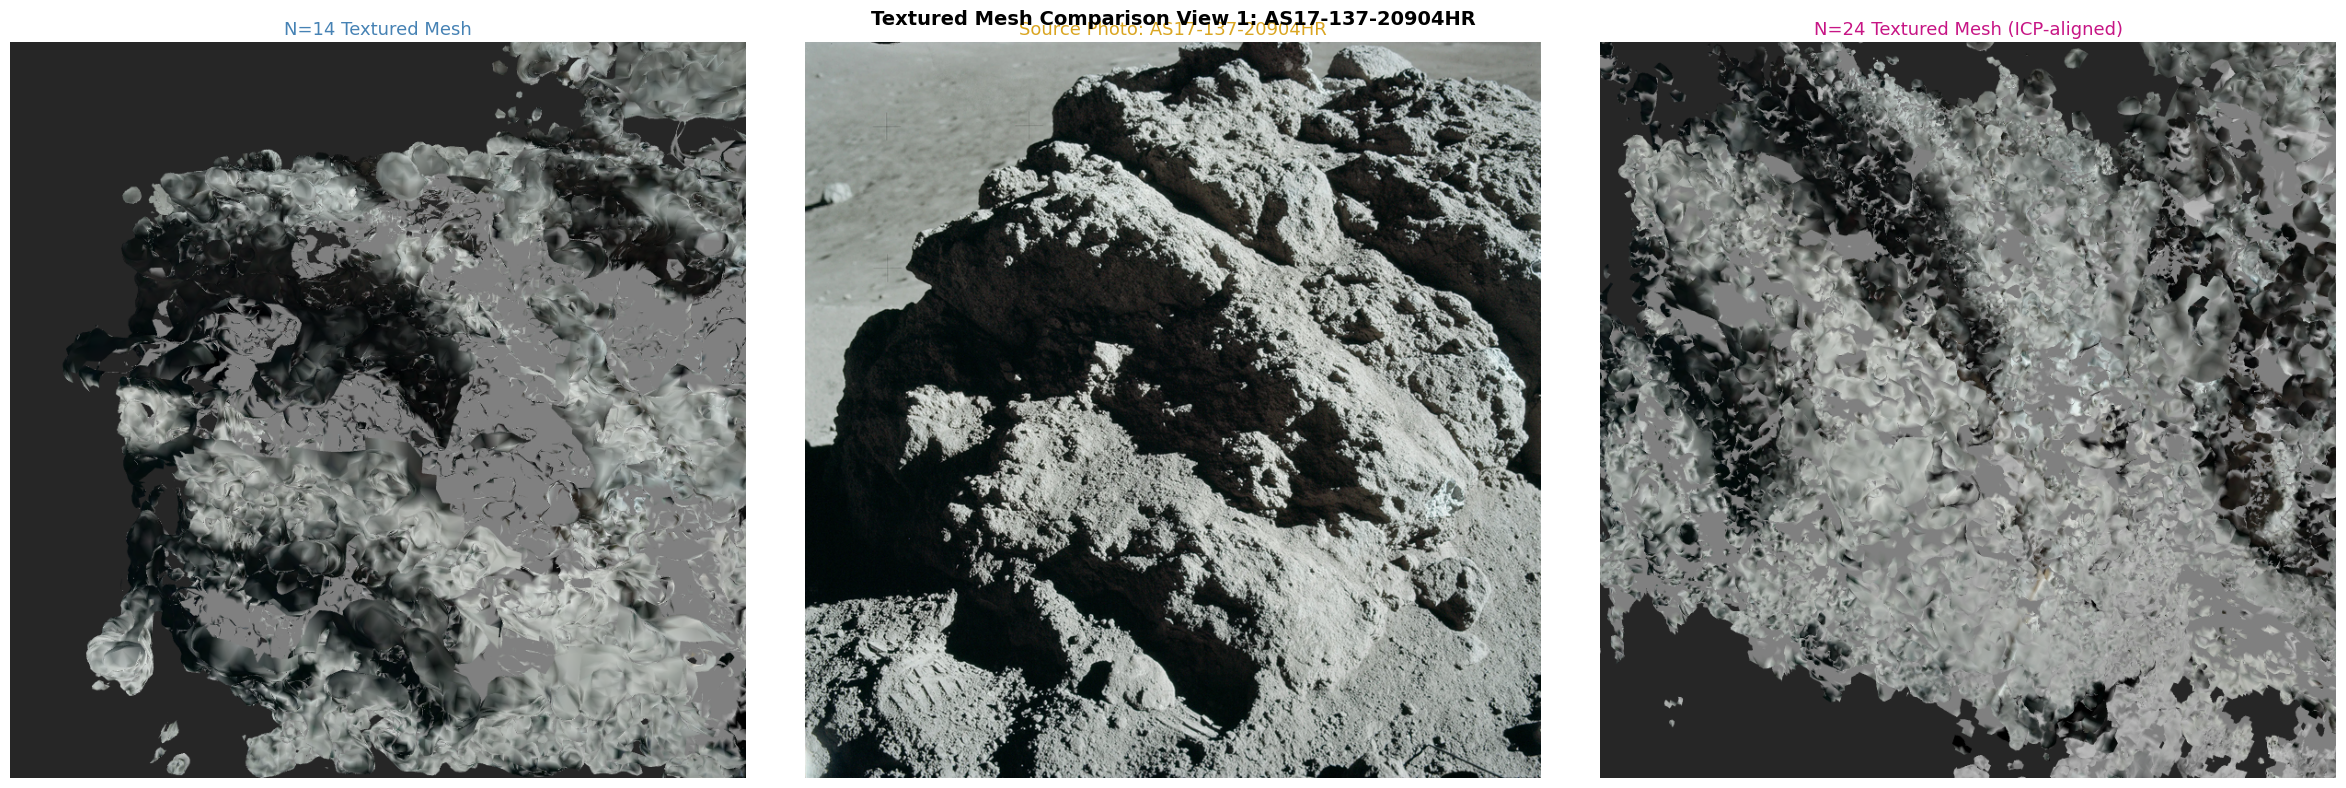
\includegraphics[width=0.9\textwidth]{../comparison/textured_sidebyside_view1.png}
    \caption{Side-by-side textured mesh comparison at view 1 (AS17-137-20904HR viewpoint, mag137 boulder). Left panel shows the N=14 textured mesh; center panel shows the original photograph; right panel shows the N=24 textured mesh. Both meshes reconstruct the main rock shape faithfully.}
    \label{fig:textured_view1}
\end{figure}

\begin{figure}[H]
    \centering
    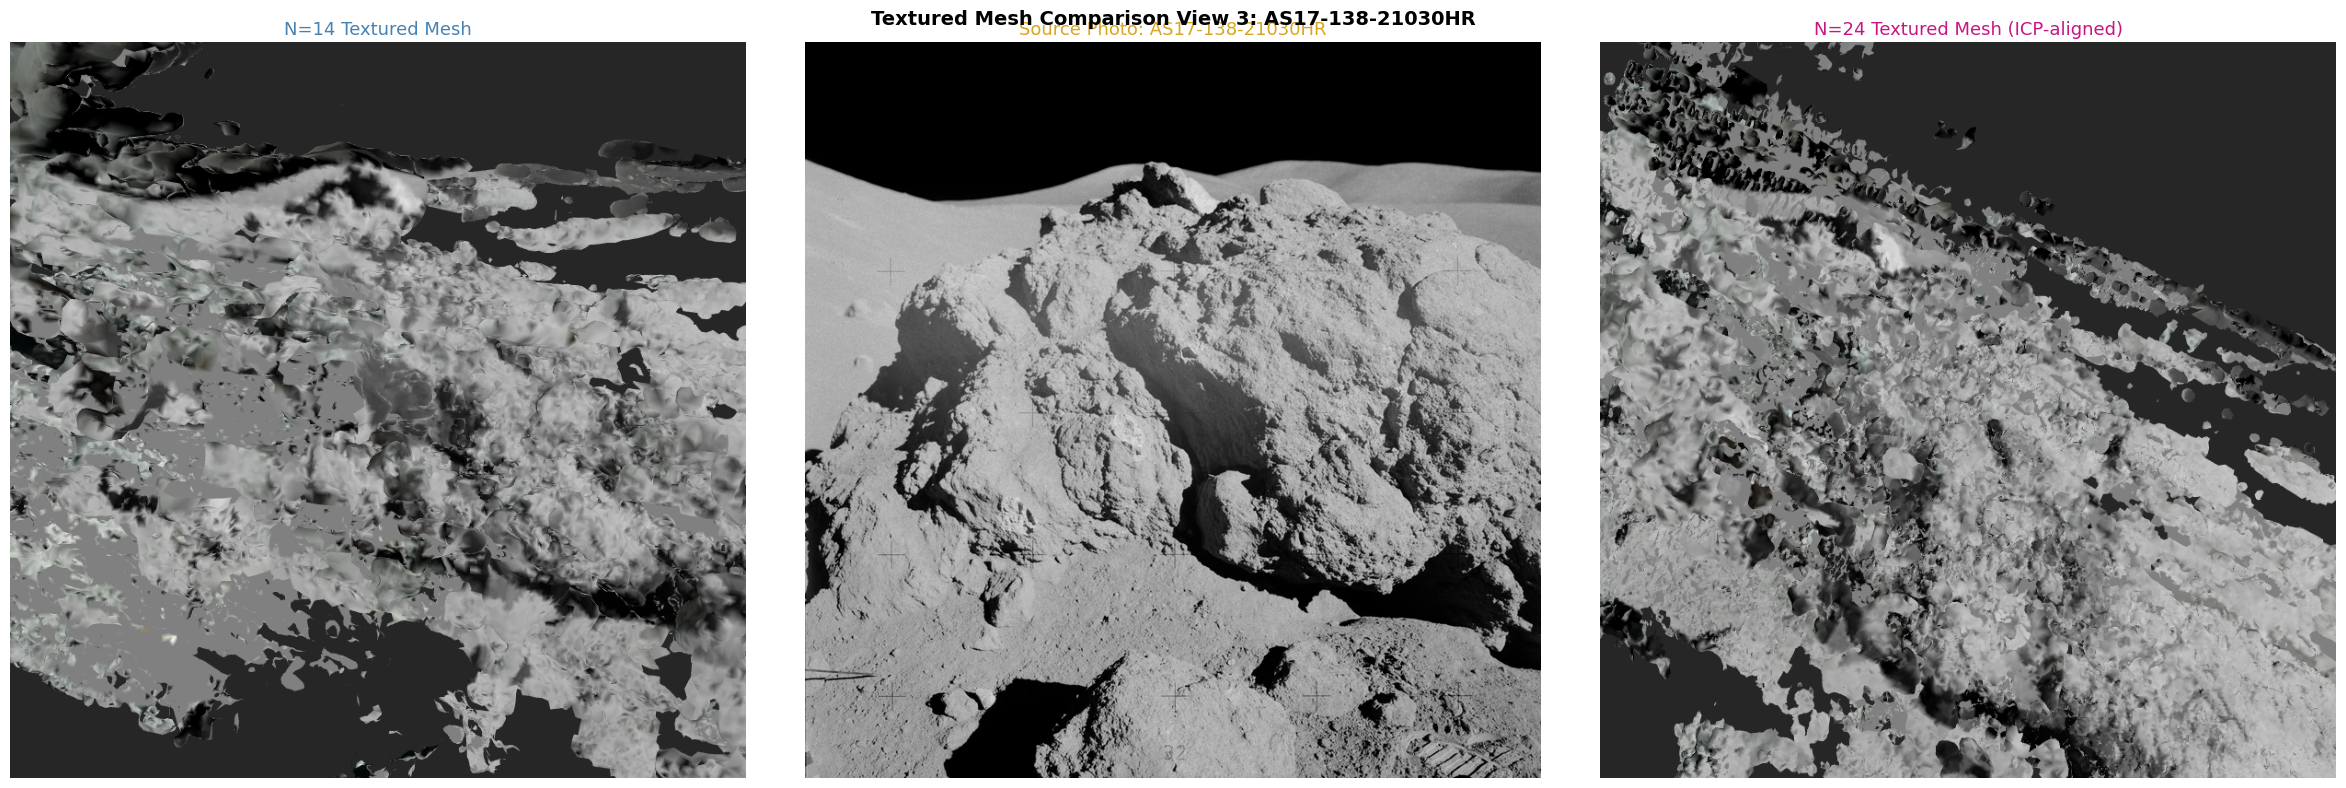
\includegraphics[width=0.9\textwidth]{../comparison/textured_sidebyside_view3.png}
    \caption{Side-by-side textured mesh comparison at view 3 (AS17-138-21030HR viewpoint, mag138 boulder). Reseau crosses are visible in the original photograph and appear as small dark artifacts in the textured mesh at this viewpoint. The mag138 boulder has lower per-vertex coverage due to the oblique camera geometry of that cluster.}
    \label{fig:textured_view3}
\end{figure}

%% ============================================================
%% Consolidated Results Summary Tables
%% ============================================================
\FloatBarrier
\subsection*{Consolidated Results Summary}

\begin{table}[H]
\centering
\caption{Summary comparison of N=14 and N=24 reconstruction pipelines.}
\label{tab:summary}
\begin{tabular}{lll}
\toprule
Quantity & N=14 & N=24 \\
\midrule
Registered images & 14 of 15 & 14 of 24 \\
Novel views registered & --- & 0 of 10 \\
Sparse 3D points & 12,769 & 12,822 \\
Fused dense points (fused.ply) & 1,641,050 & 2,453,709 \\
Poisson mesh vertices & 1,063,577 & 4,658,194 \\
Poisson mesh faces & 2,121,270 & 9,375,366 \\
Textured coverage (per-vertex) & 21.19\% & 12.22\% \\
Splatfacto mean PSNR & 33.93~dB & n/a \\
Splatfacto mean SSIM & 0.943 & n/a \\
\bottomrule
\end{tabular}
\end{table}

\begin{table}[H]
\centering
\caption{Quantitative comparison metrics (N=14 vs N=24, all values from comparison/quantitative\_metrics.json).}
\label{tab:metrics_summary}
\begin{tabular}{ll}
\toprule
Metric & Value \\
\midrule
ICP fitness & 0.065 \\
ICP inlier RMSE (COLMAP units) & 0.01518 \\
Chamfer distance (COLMAP units) & 0.219 \\
Hausdorff p99 (COLMAP units) & 2.127 \\
F-score at 1\% diagonal & 0.673 \\
F-score at 5\% diagonal & 0.934 \\
F-score at 10\% diagonal & 0.984 \\
\bottomrule
\end{tabular}
\end{table}

%% ============================================================
\section{Discussion}
\label{sec:discussion}
%% ============================================================

\subsection{Why the Novel Views Failed Registration}
\label{subsec:registration_failure}

The failure of all 10 novel views to register in COLMAP is not due to a lack of two-dimensional feature matches. Table~\ref{tab:novel_registration} shows 852--8,123 inlier matches per novel image against the 23 other images. The failure occurs at the step from two-dimensional to three-dimensional correspondences.

COLMAP's PnP-based image registration requires 2D--3D correspondences: keypoints in the new image must match keypoints that are already triangulated into the sparse model. The existing sparse model's 3D points were created by triangulating SIFT keypoints extracted from the 14 original photographic images. A rendered image from the splatfacto model generates SIFT keypoints at pixel positions that differ subtly from the photographic originals because:

\begin{enumerate}
    \item \textbf{Rendering smoothness:} The 3DGS rasterizer produces spatially smooth radiance fields. Thin high-contrast edges in the rock photographs (grain boundaries, shadow edges) are represented by Gaussian mixtures that produce slightly softer edge responses. SIFT detects scale-space extrema at positions determined by Laplacian-of-Gaussian peaks; a blurred edge shifts the peak by 0.5--3 pixels.
    \item \textbf{Absence of film grain:} Photographic film grain contributes high-frequency texture that SIFT responds to. The Gaussian model averages over grain instances visible in all training views but does not reproduce grain-level stochasticity in novel views, removing a class of high-frequency keypoints from the rendered images.
    \item \textbf{Tone mapping:} The splatfacto model applies an exposure and tone mapping correction during training. Novel views are rendered with the learned affine color correction, which may differ slightly from the photographic paper scan's gamma, altering absolute pixel values and shifting the local contrast structure that drives SIFT extrema.
\end{enumerate}

The consequence is that the 2D--2D matches between rendered and photographic images land at keypoints that are NOT in the existing 3D point tracks. COLMAP finds the 2D correspondences (both SIFT descriptor vectors are similar enough to match) but cannot promote them to 2D--3D correspondences (the matched photographic keypoint was never triangulated). From COLMAP's perspective, the novel view sees zero existing 3D landmarks, and PnP fails.

The statistic that most clearly demonstrates this mechanism is the asymmetry in Table~\ref{tab:novel_registration}: the mag137 novel views show large inlier match counts (4,422--8,123) while the mag138 novel views show much smaller counts (852--1,590). The mag138 originals have lower PSNR (though still good: 33--37~dB), which means the rendered mag138 novel views have subtly more appearance difference from the photographic mag138 originals, suppressing the number of descriptor-level matches.

\subsection{What Actually Caused the N=24 Mesh Density Increase}

The $N{=}24$ Poisson mesh has 4,658,194 vertices versus 1,063,577 for $N{=}14$ --- a 4.38$\times$ increase. Because zero novel views registered, this increase cannot come from new geometric observations. The actual source is the two-stage Poisson reconstruction applied to the $N{=}24$ dense cloud.

The $N{=}14$ pipeline used Poisson depth~9. The $N{=}24$ pipeline's first Poisson attempt (also at depth~10 but on the full cloud without background filtering) produced only 88,049 vertices due to the inflated bounding box from background outlier points. After applying the cluster-proximity filter (retaining only points within 10 COLMAP units of either cluster centroid), the bounding box contracted from $\sim$80 COLMAP units in $Z$ to $\sim$14 COLMAP units. At depth~10 with a contracted bounding box, the octree grid resolution increased to approximately 0.014 COLMAP units per cell, enabling the Poisson solver to resolve surface detail at a finer scale than the $N{=}14$ depth-9 mesh.

In other words, the density improvement is an artifact of the difference in Poisson reconstruction parameters (background filtering and octree depth) rather than additional coverage from novel views. The $N{=}24$ mesh is geometrically denser than $N{=}14$ but reconstructs the same surface from the same 14 cameras. The F-score@5\% = 0.934 confirms that the two surfaces are broadly co-located; the F-score@1\% = 0.673 reflects the fine-scale surface position differences that arise from the different Poisson resolution.

\subsection{The Null Result as a Contribution}

The outcome that 0 of 10 novel views registered is a useful, reproducible negative result. It establishes a precise boundary: out-of-the-box COLMAP with SIFT feature matching cannot use 3DGS-rendered novel views as photogrammetric observations on this class of dataset. This is not a trivial failure mode; prior literature has not systematically tested this specific pipeline composition, and the failure mechanism (keypoint-position mismatch at the 2D-to-3D promotion step) is now precisely identified.

The natural follow-up is to replace SIFT with a learned feature matcher. SuperPoint+SuperGlue, LightGlue, and LoFTR all use neural descriptors trained to be robust to appearance differences of the kind introduced by neural rendering. Dense correspondence methods (DKM, RoMa) match every pixel without relying on repeatable keypoint detection, which would eliminate the keypoint-position mismatch entirely. Any of these approaches would likely succeed where SIFT failed, and the present work provides the experimental baseline against which that improvement can be measured.

\subsection{Caveats from the Phase 2 Report}

Three important caveats from the analysis in \texttt{comparison/PART\_B\_PHASE\_2\_REPORT.md} deserve explicit restatement:

\textbf{Caveat 1 --- Learned descriptors.} The registration failure is specific to SIFT, not to the splat-augmentation concept. A different feature matching strategy (SuperPoint/SuperGlue, learned descriptors) might successfully match rendered views to photographic keypoints, enabling registration. The hypothesis that rendered novel views can augment photogrammetric reconstruction remains viable; it has simply not been confirmed for SIFT-based matching on this dataset.

\textbf{Caveat 2 --- Scene geometry constraint.} The two-cluster geometry (8.66-unit inter-cluster distance, 7 cameras per cluster) means the pose graph is already strongly constrained by the original 14 cameras. Even if novel views registered, they would add density within the existing viewing envelope rather than extending it to new surface areas. A single-cluster dataset (all images of one rock) would be a better testbed for the splat-augmentation hypothesis: coverage gaps are larger, and novel views from oblique or top-down angles would genuinely add new surface coverage.

\textbf{Caveat 3 --- ICP fitness and mesh topology.} The ICP fitness of 0.065 (6.5\% inlier correspondence rate) reflects both the mesh topology mismatch between 1.06M and 4.66M vertex meshes and the residual rotation (approximately $17^\circ$) between independent bundle adjustments. This low fitness means that the ICP result may not represent the true optimal alignment between the two surfaces; a correspondence-free alignment method (e.g., multi-resolution ICP with larger initial correspondence distance) might reduce the Hausdorff p99 from 2.127 units.

\subsection{Per-Vertex Texturing Tradeoffs}

The coverage rates of 21.19\% (N=14) and 12.22\% (N=24) are bounded above by the field of view of the 14 registered cameras. The per-vertex projection algorithm correctly handles occlusion via ray-casting, so uncolored vertices are genuinely invisible to every camera, not a defect in the algorithm.

The ceiling for coverage under the current camera set can be estimated from the solid angle subtended by the 14 cameras. The two clusters are each photographed from $\approx 7$ cameras spanning roughly $\pm 30^\circ$ in azimuth. This means the top, underside, and lateral flanks of each boulder are not seen by any camera, placing a physical upper bound on textured coverage of approximately 35--45\% for this scene.

A UV atlas approach using texrecon would not raise the physical coverage ceiling but would produce sharper texture boundaries (no per-vertex color discontinuities) and support normal-mapped rendering. The texrecon tool requires a watertight or near-watertight UV parameterization; the xatlas library that was attempted requires 45+ minutes per mesh at $>$2M faces on the available hardware. A mesh simplification step to $\lesssim$500K faces before UV parameterization, followed by texture reprojection and upsampling, is the recommended path for a Tier A textured deliverable in future work.

%% ============================================================
\section{Conclusion}
\label{sec:conclusion}
%% ============================================================

This project delivered a complete photogrammetric reconstruction pipeline for the Apollo 17 boulder scene, from raw Hasselblad photographs to per-vertex textured meshes, with quantitative validation via three independent geometric metrics. The specific outcomes are:

\textbf{Photogrammetric pipeline:} Fully complete to textured mesh for both $N{=}14$ and $N{=}24$ datasets. The $N{=}14$ baseline mesh has 1,063,577 vertices; the $N{=}24$ mesh has 4,658,194 vertices. Both are stored as per-vertex colored PLY files in \texttt{colmap\_n15/dense/textured/} and \texttt{colmap\_n24/dense/textured/} respectively.

\textbf{Splatfacto model:} Successfully trained to 30,000 iterations with $\approx$993,000 Gaussians. Mean PSNR 33.93~dB, mean SSIM 0.943 over all 14 training views.

\textbf{Novel-view synthesis:} 10 non-blank novel views generated (5 per magazine cluster, $\pm 30^\circ$ azimuth arc). All frames validated with pixel standard deviation $> 43$.

\textbf{Augmentation hypothesis:} Tested and rejected on this dataset under SIFT-based feature matching. Zero of 10 novel views registered in COLMAP despite 852--8,123 two-dimensional inlier matches per image. The failure mechanism is the inability to promote 2D--2D matches to 2D--3D correspondences against the existing sparse model.

\textbf{Quantitative comparison:} F-score@5\% = 0.934 establishes that the two reconstructions agree on 93.4\% of their surface samples within 5\% of the scene extent. The Chamfer distance of 0.219 COLMAP units ($\approx 1.35\%$ of the bounding box diagonal) confirms close geometric consistency.

The project documents a concrete, reproducible experimental result: SIFT-based COLMAP cannot leverage 3DGS-rendered novel views for photogrammetric augmentation on this dataset, and the identified failure mechanism points directly to learned feature matching as the necessary next step.

%% ============================================================
%% Appendix
%% ============================================================
\clearpage
\appendix

\section{Untextured Geometry Baseline}

\begin{figure}[H]
    \centering
    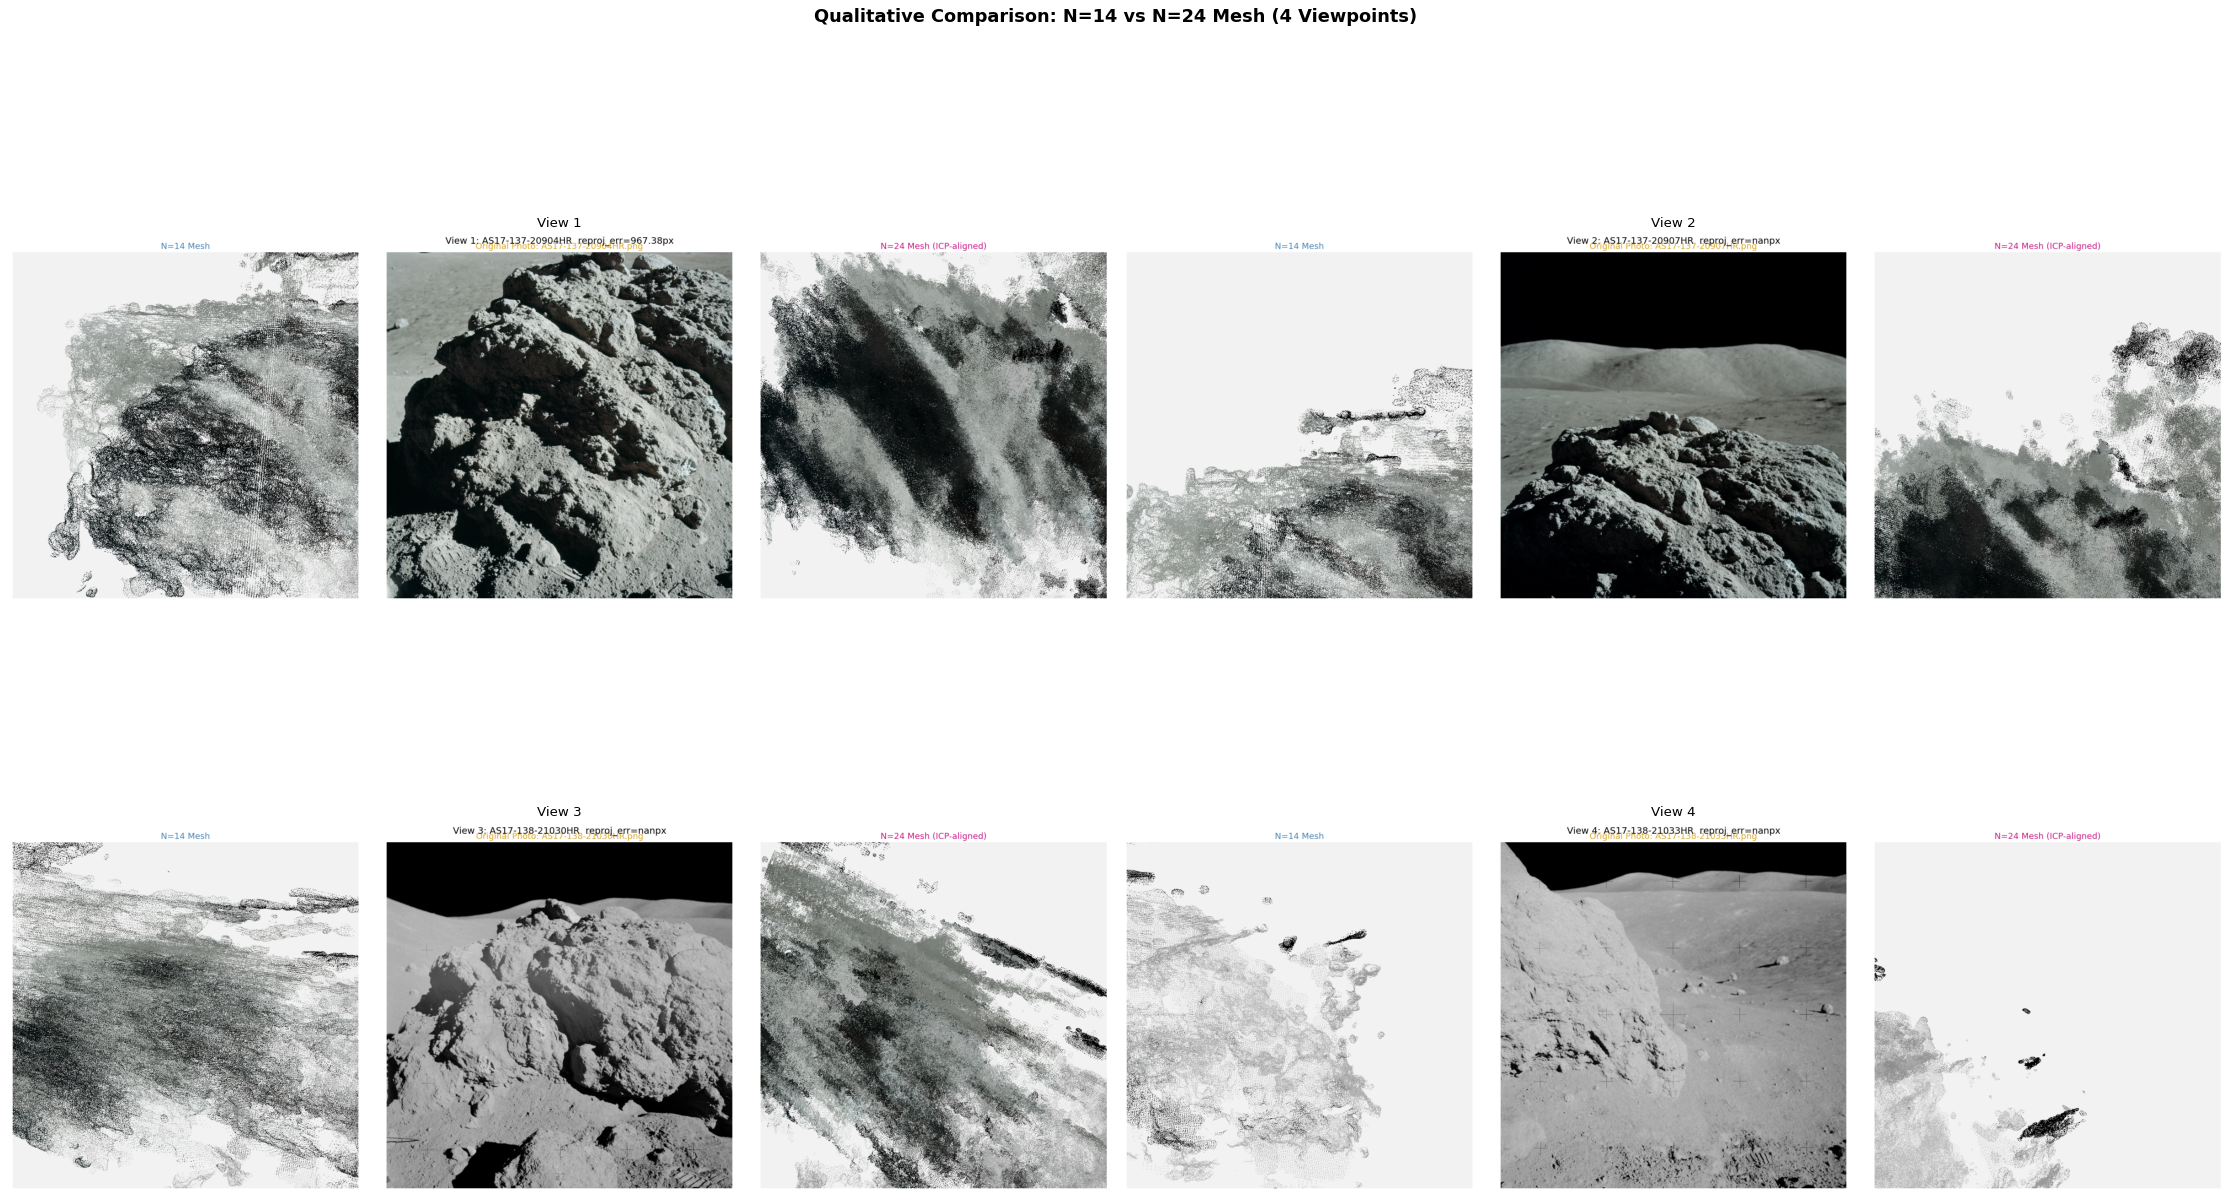
\includegraphics[width=\textwidth]{../comparison/qualitative_grid.png}
    \caption{Untextured geometry baseline: four-viewpoint comparison grid of N=14 mesh renders (left column), original photographs (center column), and N=24 mesh renders (right column) before per-vertex texturing. Comparing with Figure~\ref{fig:textured_grid} shows the improvement in surface interpretability from per-vertex color projection.}
    \label{fig:untextured_grid}
\end{figure}

%% ============================================================
\section{Code Appendix}
%% ============================================================

All Python scripts authored for this project are reproduced below in full. Scripts are grouped by function and listed alphabetically within each group. File paths are given relative to the project root (\texttt{ses598-apollo17/}).

\subsection{Group A: Photogrammetry Pipeline}

\subsubsection{\texttt{build\_n24\_dataset.py}}
\lstinputlisting[language=Python, caption=build\_n24\_dataset.py]{../build_n24_dataset.py}

\subsubsection{\texttt{mvs\_dense.py} (N=14)}
\lstinputlisting[language=Python, caption=mvs\_dense.py]{../mvs_dense.py}

\subsubsection{\texttt{colmap\_n24/dense/mvs\_dense.py} (N=24 adapted)}
\lstinputlisting[language=Python, caption=colmap\_n24/dense/mvs\_dense.py]{../colmap_n24/dense/mvs_dense.py}

\subsubsection{\texttt{preprocess.py}}
\lstinputlisting[language=Python, caption=preprocess.py]{../preprocess.py}

\subsubsection{\texttt{refine\_mesh.py}}
\lstinputlisting[language=Python, caption=refine\_mesh.py]{../refine_mesh.py}

\subsubsection{\texttt{remesh\_n24.py}}
\lstinputlisting[language=Python, caption=remesh\_n24.py]{../remesh_n24.py}

%% ============================================================
\subsection{Group B: Comparison and Evaluation}

\subsubsection{\texttt{check\_registered.py}}
\lstinputlisting[language=Python, caption=check\_registered.py]{../check_registered.py}

\subsubsection{\texttt{compare\_21036.py}}
\lstinputlisting[language=Python, caption=compare\_21036.py]{../compare_21036.py}

\subsubsection{\texttt{compute\_metrics.py}}
\lstinputlisting[language=Python, caption=compute\_metrics.py]{../compute_metrics.py}

\subsubsection{\texttt{mesh\_compare.py}}
\lstinputlisting[language=Python, caption=mesh\_compare.py]{../mesh_compare.py}

\subsubsection{\texttt{qualitative\_compare.py}}
\lstinputlisting[language=Python, caption=qualitative\_compare.py]{../qualitative_compare.py}

\subsubsection{\texttt{recover\_21036.py}}
\lstinputlisting[language=Python, caption=recover\_21036.py]{../recover_21036.py}

%% ============================================================
\subsection{Group C: Novel-Pose Synthesis and Rendering}

\subsubsection{\texttt{diagnose\_novel.py}}
\lstinputlisting[language=Python, caption=diagnose\_novel.py]{../diagnose_novel.py}

\subsubsection{\texttt{gen\_novel\_poses.py}}
\lstinputlisting[language=Python, caption=gen\_novel\_poses.py]{../gen_novel_poses.py}

\subsubsection{\texttt{make\_contact\_sheet.py}}
\lstinputlisting[language=Python, caption=make\_contact\_sheet.py]{../make_contact_sheet.py}

\subsubsection{\texttt{novel\_pose\_smoke.py}}
\lstinputlisting[language=Python, caption=novel\_pose\_smoke.py]{../novel_pose_smoke.py}

\subsubsection{\texttt{sanity\_render.py}}
\lstinputlisting[language=Python, caption=sanity\_render.py]{../sanity_render.py}

\subsubsection{\texttt{test\_novel\_per\_magazine.py}}
\lstinputlisting[language=Python, caption=test\_novel\_per\_magazine.py]{../test_novel_per_magazine.py}

%% ============================================================
\subsection{Group D: Texturing and Qualitative Comparison}

\subsubsection{\texttt{make\_comparison\_grid.py}}
\lstinputlisting[language=Python, caption=make\_comparison\_grid.py]{../make_comparison_grid.py}

\subsubsection{\texttt{qualitative\_compare\_textured.py}}
\lstinputlisting[language=Python, caption=qualitative\_compare\_textured.py]{../qualitative_compare_textured.py}

\subsubsection{\texttt{texture\_mesh\_uv.py}}
\lstinputlisting[language=Python, caption=texture\_mesh\_uv.py]{../texture_mesh_uv.py}

\subsubsection{\texttt{texture\_mesh\_vertex.py}}
\lstinputlisting[language=Python, caption=texture\_mesh\_vertex.py]{../texture_mesh_vertex.py}

\end{document}
